%%
%% Author: novitoll
%% 3/9/18
%%

% Preamble
\documentclass[11pt]{article}

% Packages
\usepackage{amsmath}
\usepackage{enumitem}
\usepackage{graphicx}
\usepackage{listings}

\graphicspath{ {pics/} }
\lstset{language=Python}
\lstset{%
  escapeinside={(*}{*)},%
}

\title{CVT: Lecture 7}
\date{2018-03-09}
\author{Novitoll}

\begin{document}
    \maketitle
    \pagenumbering{arabic}

    \section{Machine learning} \label{sec:mlintro}

    \begin{itemize}
        \item Supervised learning
        \item Unsupervised learning
        \item Reinforcement learning
    \end{itemize}

    \section{Linear regression} \label{sec:linearreg}

    Simple linear function $y = mx + b$ in Supervised Learning has the hypothesis $h_\theta(x) = \theta_0 + \theta_1 x$
    to predict with given X N-dimensional matrix of features, $\theta$ is coefficient (something to be found during model training)

    \[
        h_\theta(x) = \theta_0 + \theta_1 x_1 + \theta_2 x_2 + .. + \theta_i x_i = \sum_{i=0}^{m} \theta_i x_i = \theta^T x
    \]

    , where $m$ - is number of features.

    Now we want to minimize the difference between hypothesis $h_\theta(x)$ and ground truth $y$ for high accuracy,
    the difference is called Cost function - $J(\theta)$.

    \[
        J(\theta) = \frac{1}{2}\sum_{i=0}^{m} (h_\theta(x^i) - y^i)^2
    \]

    This is the generalized cost function, in practice you will find its implementations as:
    \begin{itemize}
        \item mean squared error (MSE) = $\frac{1}{2m}\sum_{i=0}^{m}..$
        \item hinge loss
        \item log loss
        \item ..
    \end{itemize}

    In order to $\min_{\theta} J(\theta)$ let's differentiate it (keeping in mind that X - is a matrix of independent variables):

    \begin{gather*}
        \frac{\partial{}}{\partial{\theta_i}}J(\theta) = \frac{\partial{}}{\partial{\theta_i}} \
            \frac{1}{2}(h_\theta(x) - y)^2 = \\
            2 \ \frac{1}{2} \frac{\partial{}}{\partial{\theta_i}} \ (h_\theta(x) - y) \
            \frac{\partial{}}{\partial{\theta_i}} \ (h_\theta(x) - y) = \\
            (h_\theta(x) - y) \ \frac{\partial{}}{\partial{\theta_i}} (\theta_0 + \theta_1 x_1 + .. + \theta_n - y) = \\
            (h_\theta(x) - y) \ \frac{\partial{}}{\partial{\theta_i}} (h_\theta(x) - y) = \\
            (h_\theta(x) - y) \ x_i
    \end{gather*}

    Update of our cost function (Batch gradient descent) is:
    \begin{align}
        \theta_i := \theta_i - \alpha \sum_{i=0}^{m} (h_\theta(x^i) - y^i) \ x^i
    \end{align}

    , where $\alpha$ - is learning rate.
    BGD (1) is good for small dataset and always finds the local minima, however with the real world dataset it's slow.
    For that, usually Stochastic gradient descent (SGD) is used:

    \begin{lstlisting}
        Repeat 1..10 {
            for j=1 .. to m {(*\begin{align}
                    \theta_i := \theta_i - \alpha (h_\theta(x^j) - y^j) \ x_i^j
                \end{align}*)
            }
        }
    \end{lstlisting}

    SGD works well with big dataset, however wont converge to the 0 (minima), but though will be close as much as possible.
    The idea is to find global minima in order not to \textbf{overfit} with finding local minima.

    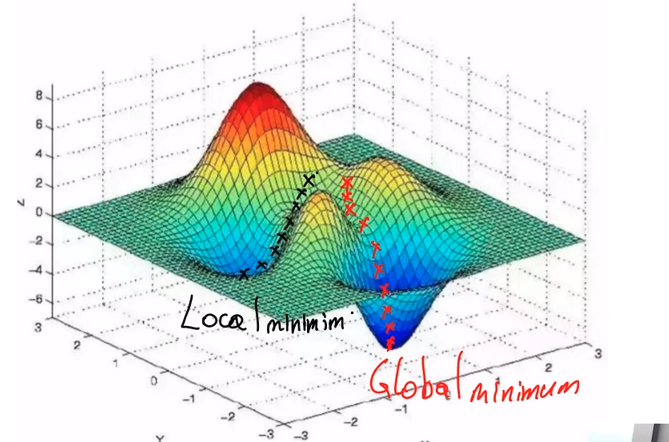
\includegraphics[scale=0.5]{sgd.png}

\end{document}